\documentclass{article}
\usepackage{graphicx} % Required for inserting images

\title{PS1}
\author{Donovan Thompson }
\date{September 2023}

\begin{document}

\maketitle
\section{Personal Statement}
\paragraph{}
In Computational Physics, my goal is to further develop my Python programming skills, particularly in the context of data analysis for laboratory experiments. With a foundation in physics and mathematics, I'm already comfortable with Python. After completing my degree, I'm considering graduate studies in physics with a theoretical emphasis, where I plan to leverage my programming skills in Python for data analysis in research 
projects. Github username is dkt9447
\section{Gaussian figure}
\begin{figure}
    \centering
    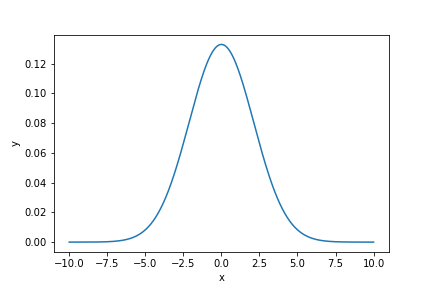
\includegraphics[width=\textwidth,height=\textheight,keepaspectratio]{gaussian.png}
    \caption{Gaussian Figure}
    \label{fig:enter-label}
\end{figure}
\end{document}


